\begin{frame}{Aufgabe 1\dots?}\onslide<+->
    \begin{exercise}
        Stellen Sie den Text \enquote{Ist das schwierig?} im ASCII-Format als Dezimal-, Binär- und Hexadezimalzahlen dar.
    \end{exercise}
    \begin{solve}[Laaaaaangweilig \texttwemoji{roll_eyes}]
        \onslide<+->\begin{tikzpicture}[overlay]
            \node[align=left,below left=2cm of current page.east] {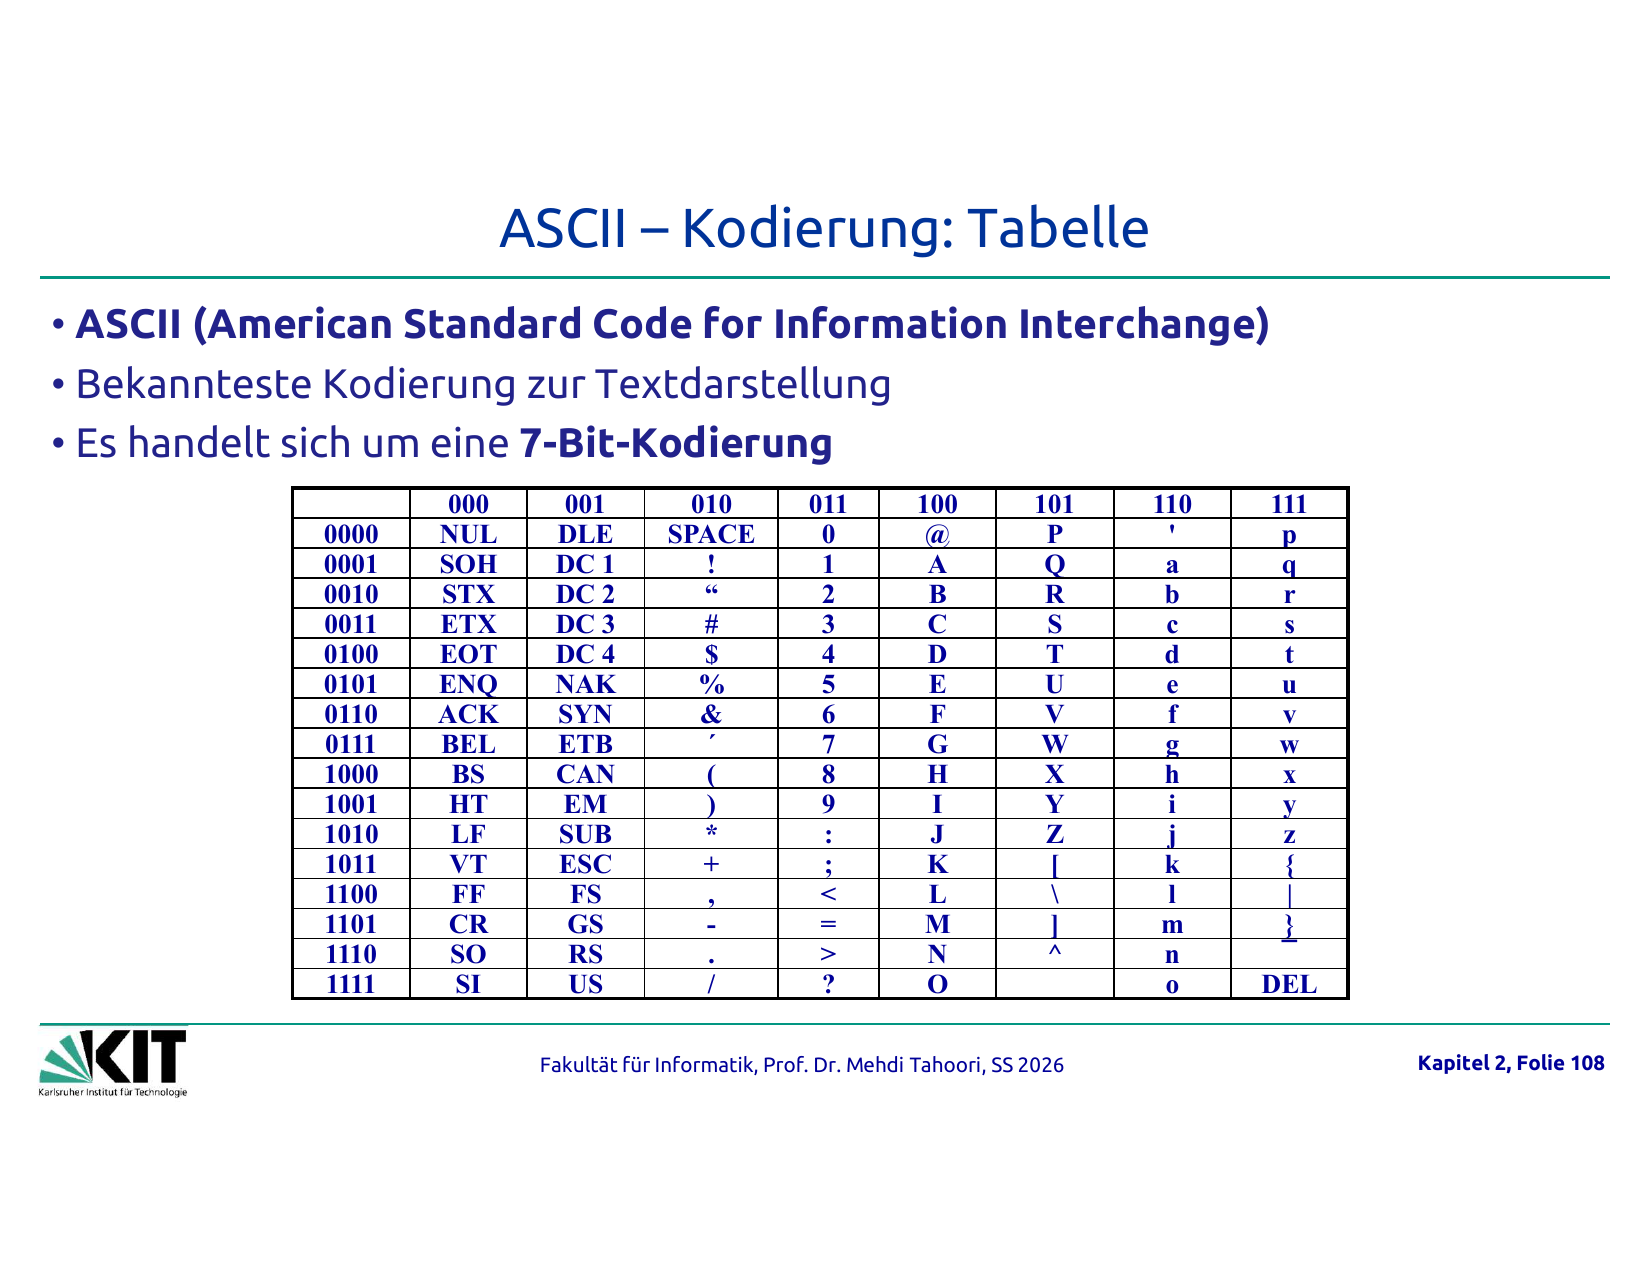
\includegraphics[scale=0.2]{slide12.png}};
        \end{tikzpicture}
        \vspace*{-\baselineskip}
        \begin{itemize}
            \item \(1001001\onslide<+->~1110011\onslide<+->~1110100\onslide<+->~\alt<.>{\mathbf{0}}{0}100000\onslide<+->~\dots \)
            \item \(0x49~0x73~0x74~0x20~\dots \)% chktex 29
            \item \(73~115~116~32~\dots \)
        \end{itemize}
    \end{solve}
\end{frame}
\begin{frame}{Vielleicht geht es ja auch einfacher\dots}
    \begin{exercise}[\enquote{Ist das schwierig?} \faAngleRight~ASCII (Dec, Bin, Hex)]\end{exercise}
    \begin{solve}[Trickserei!]
        Schauen wir uns das mal genauer an:
        \begin{itemize}
            \item<2-> \(\mathtt{'a'}={\only<6->{\color{purple}}011}0~0001_{(2)}=97_{(10)}\)
            \item<4-> \(\mathtt{'b'}={\only<6->{\color{purple}}011}0~0010_{(2)}=98_{(10)}\)
            \item<6-> \(\cdots \)
            \item<3-> \(\mathtt{'A'}={\only<6->{\color{purple}}010}0~0001_{(2)}=65_{(10)}\)
            \item<5-> \(\mathtt{'B'}={\only<6->{\color{purple}}0\tikzmark{binmark0}10}0~0010_{(2)}=66_{(10)}\)
            \item<6-> \(\cdots \)
        \end{itemize}
    \end{solve}
    \onslide<6->\begin{tikzpicture}[overlay,remember picture]
        \node [inner sep=0,below right = 0.05cm and 2pt of pic cs:binmark0] (n0) {};
        \node [inner sep=2pt,below right = 0em and 12em of pic cs:binmark0,draw=purple,rounded corners] (n1) {\begin{minipage}{0.5\textwidth}
            \centering\scriptsize Da unser Alphabet \(26_{(10)}=11010_{(2)}\) Buchstaben\\hat, müssen wir \(5\) Stellen rechts freihalten!
        \end{minipage}};
        \node [inner sep=0,below left = -0.35cm and 0.05cm of n1] (n2) {};
        \draw (n0) edge[->,bend right=20] (n2);
    \end{tikzpicture}
\end{frame}

\addtocounter{exercise}{-1}\addtocounter{solve}{-1}
\begin{frame}[noframenumbering]{Vielleicht geht es ja auch einfacher\dots}
    \begin{exercise}[\enquote{Ist das schwierig?} \faAngleRight~ASCII (Dec, Bin, Hex)]\end{exercise}
    \begin{solve}[Trickserei!]
        Das heißt:\begin{itemize}
            \item<2-> Kleinbuchstaben: \(\textcolor{purple}{011}0\only<4|handout:0>{\mathllap{\underbrace{\hphantom{0110}}_\text{\color{lightgray}0x\color{blue}6}}}~0001\only<4|handout:0>{\mathllap{\underbrace{\hphantom{0001}}_\text{\color{lightgray}0x\color{blue}1}}}\)~---~\(\textcolor{purple}{011}1\only<4|handout:0>{\mathllap{\underbrace{\hphantom{0111}}_\text{\color{lightgray}0x\color{blue}7}}}~1010\only<4|handout:0>{\mathllap{\underbrace{\hphantom{1010}}_\text{\color{lightgray}0x\color{blue}A}}}\)\only<4|handout:0>{\vspace{-3pt}}\\
            \hphantom{Kleinbuchstaben: }\only<5->{\(\color{lightgray}0x\color{blue}61\)~---~\(\color{lightgray}0x\color{blue}7A\)}\\
            \hphantom{Kleinbuchstaben: }\only<6->{\(97\)~---~\(122\)}
            \item<3-> Großbuchstaben: \(\textcolor{purple}{010}0\only<4|handout:0>{\mathllap{\underbrace{\hphantom{0100}}_\text{\color{lightgray}0x\color{blue}4}}}~0001\only<4|handout:0>{\mathllap{\underbrace{\hphantom{0001}}_\text{\color{lightgray}0x\color{blue}1}}}\)~---~\(\textcolor{purple}{010}1\only<4|handout:0>{\mathllap{\underbrace{\hphantom{0101}}_\text{\color{lightgray}0x\color{blue}5}}}~1010\only<4|handout:0>{\mathllap{\underbrace{\hphantom{1010}}_\text{\color{lightgray}0x\color{blue}A}}}\)\only<4|handout:0>{\vspace{-3pt}}\\
            \hphantom{Großbuchstaben: }\only<5->{\(\color{lightgray}0x\color{blue}41\)~---~\(\color{lightgray}0x\color{blue}5A\)}\\
            \hphantom{Großbuchstaben: }\only<6->{\(65\)~---~\(90\)}
        \end{itemize}
    \end{solve}
\end{frame}